\documentclass[12pt]{report}
\usepackage[utf8x]{inputenc}
\usepackage{graphicx}
\usepackage{gensymb}
\usepackage{algorithm}
\usepackage[noend]{algpseudocode}
\usepackage{algpseudocode}
\graphicspath{ {./images/} }
\usepackage{fancyhdr}
\usepackage[T1]{fontenc}


\title{ETERNITY: FUNCTION}								
\author{Pragya Tomar}						
\date{}

\makeatletter
\let\thetitle\@title
\let\theauthor\@author
\let\thedate\@date
\makeatother

\pagestyle{fancy}
\fancyhf{}
\rhead{\thetitle}
\cfoot{\thepage}

\begin{document}

\begin{titlepage}
	\centering
    \vspace*{1 cm}
\begin{center}    \textsc{\Large Concordia University}\\[2.5 cm]
{Problem 1 }\\[0.4 cm]
\end{center}
	\textsc{\Large  SOEN 6011 - Software Engineering Process }\\[1 cm]
	\rule{\linewidth}{0.5 mm} \\[0.4 cm]
	{ \huge \textbf \thetitle}\\[0.5 cm]
	{ \huge \textbf{($\sigma$)}}
	\rule{\linewidth}{0.5 mm} \\[1.0 cm]

	
\begin{center}   {\Large \textbf{\theauthor}} \\[1 cm]
                 {\large Student ID : 40197757 }\\[0.4 cm]
                 {\large Repository Address: https://github.com/pragya231/SOEN6011}
\end{center}
	
\end{titlepage}

\tableofcontents
\pagebreak

\renewcommand{\thesection}{\arabic{section}}
\section{\Large \vspace{0.1 cm}Introduction}

\subsection{\Large \vspace{0.1 cm}Description}
The standard deviation gives a measure of the amount of dispersion for a given set of values and is calculated as a square root of variance. The standard deviation function is denoted by a lower case Greek letter sigma $\sigma$.

\begin{figure}[h!]
\begin{center}
  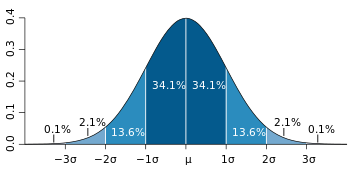
\includegraphics[width=6cm, height=3cm]{Standard_deviation_diagram.svg_.png}
  \end{center}
  \caption{Graph of standard deviation function (Source: Google Images)}
\end{figure}

It is calculated as given below:

$$Standard Deviation = {\Large\sqrt{ \frac{\sum_{i=1}^{n}(x_i-\overline x)^2}{n-1}}}$$


\subsection{\Large \vspace{0.1 cm}Domain}
The domain of the sigma($\sigma$) function is all the real number (-$\infty$,+$\infty$).

\subsection{\Large \vspace{0.1 cm}Co-Domain}
The co-domain of the sigma($\sigma$) function is (0,$+\infty$).  
 
\subsection{\Large \vspace{0.1 cm}Unique Characteristics}
\begin{itemize}
    \item It measures dispersion of dataset relative to its mean.
    \item Function is expressed in same units as the data.
    \item The higher standard deviation indicates the data set are spread over the wider range. 
\end{itemize}

\subsection{\Large\vspace{0.4 cm}Context of Use Model}
This is a simple basic calculator to calculate the standard deviation of a group of numbers. The users can press any key given on the calculator to enter the input. A decimal point and a negative symbol is also provided on the calculator as the input can be a real number. The calculator will then return the output or a message which indicates that the given input is invalid in order to calculate the standard deviation.

\vspace{1cm}

\begin{figure}[h!]
\begin{center}
  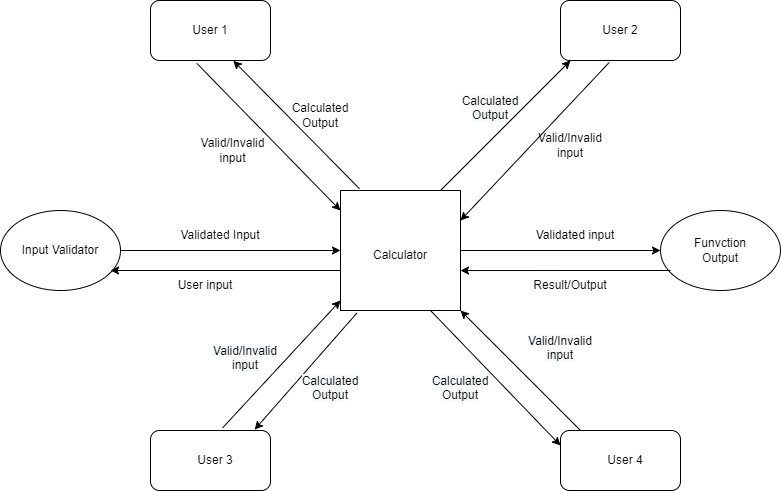
\includegraphics[width=5cm, height=7cm]{Context of Use Model.jpg} 
   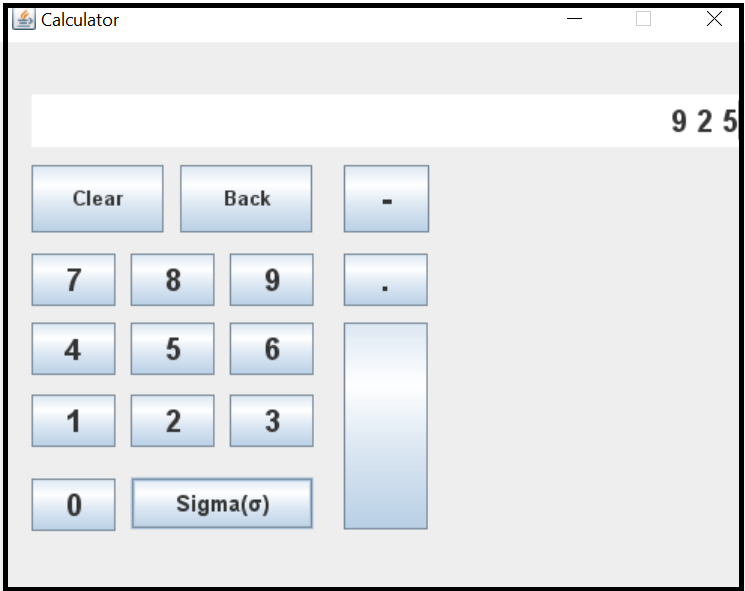
\includegraphics[width=5cm, height=7cm]{images/Graphical Interface.png} 
  \end{center}
  \caption{\vspace{0.8 cm}Graphical User Interface and Context of Use Model}
\end{figure}

\begin{thebibliography}{9}
\bibitem{Standard Deviation} 
Standard Deviation
\\\texttt{https://www.geeksforgeeks.org/how-to-find-the-standard-deviation-in-statistics/}

\bibitem{Standard Deviation in Java}
Standard Deviation in Java
\\\texttt{https://javatutoring.com/java-standard-deviation-array/}



\end{thebibliography}
\end{document}